\documentclass[aspectratio=169, 11pt]{beamer}
\usepackage[english]{babel}    % faire du français
\usepackage[T1]{fontenc}        % accents dans le DVI
\usepackage[utf8]{inputenc}   % accents dans le source
\usepackage{graphicx}
\usepackage{amssymb}
\usepackage{mathtools}
\usepackage{color, colortbl}
\usepackage{mdframed}
\usepackage{animate} %% Insert gif as png list
\usepackage{media9} %% play video/audio in frame. Use acroread to play pdf

%% Set title/author/institute
\title[Introduction au Machine Learning]{Introduction au Machine Learning}
\subtitle[Régression linéaire]{Régression linéaire}
\author{Léo Beaucourt}
\institute{Agaetis}

%% Use specific font
\usepackage{libertine}
\renewcommand*\familydefault{\sfdefault}  %% Only if the base font of the document is to be sans serif

\usefonttheme[onlymath]{serif}

%% Set frames margin
\setbeamersize{text margin left=10pt,text margin right=10pt}

%% Remove latex navigation symbols
\setbeamertemplate{navigation symbols}{}

%% Define background image
%\pgfdeclareimage[height=\textheight,width=\textwidth]{bkg}{figs/frontAgaetis}
%\setbeamertemplate{background}{\pgfuseimage{bkg}}

%% Set beamer background color
%\setbeamercolor{background canvas}{bg=black}

%% Set default text color
%\setbeamercolor{normal text}{fg=paleGray,bg=black}

%% Define frame title color
\setbeamercolor{frametitle}{fg=agaetisOrange}

%% Set items styles and colors
\setbeamercolor{itemize item}{fg=agaetisOrange}
\setbeamertemplate{itemize item}[circle]
\setbeamercolor{itemize subitem}{fg=agaetisOrange}
\setbeamertemplate{itemize subitem}[triangle]
\setbeamercolor{enumerate item}{fg=agaetisOrange}
\setbeamercolor{enumerate subitem}{fg=agaetisOrange}

%% Define personal colors
\definecolor{paleGray}{RGB}{160,160,160}
\definecolor{paleOrange}{RGB}{255,204,153}
%\definecolor{agaetisOrange}{RGB}{255,137,63}
\definecolor{agaetisOrange}{RGB}{230,74,25}
\definecolor{forestGreen}{RGB}{0,204,0}
\definecolor{veryPaleOrange}{RGB}{255,229,204}

%% Boxes prototypes
\beamerboxesdeclarecolorscheme{suppervise}{agaetisOrange}{paleOrange}
\setbeamercolor{box}{fg=black,bg=paleOrange}

%% New command to use bullet point
\newcommand{\tabitem}{~~\llap{\textbullet}~~}

%% Define footliner
\setbeamertemplate{footline}
{                  
  \leavevmode%
  \hbox{%
    \begin{beamercolorbox}[wd=.2\paperwidth,ht=2.25ex,dp=1ex,center]{author in head/foot}%
      \usebeamerfont{author in head/foot}\textcolor{agaetisOrange}{\insertshortauthor\hspace*{1em}-\hspace*{1em}\insertshortinstitute}
  \end{beamercolorbox}%
  \begin{beamercolorbox}[wd=.6\paperwidth,ht=2.25ex,dp=1ex,center]{author in head/foot}%
      \usebeamerfont{title in head/foot}\textcolor{paleGray}{\insertshorttitle}
  \end{beamercolorbox}%
  \begin{beamercolorbox}[wd=.2\paperwidth,ht=2.25ex,dp=1ex,center]{author in head/foot}%
      \textcolor{agaetisOrange}{\insertframenumber{} / \inserttotalframenumber}
  \end{beamercolorbox}}%
  \vskip0pt%
}

%%
% START DOCUMENT
%%

\begin{document}

\begin{frame}
  \begin{figure}
    
\includegraphics[width=0.5\textwidth]{figs/AGAETIS_GREY}
  \end{figure}
  \begin{center}
    \Large
    \textcolor{agaetisOrange}{\insertshorttitle}\\
    \large
    \textcolor{agaetisOrange}{\insertshortsubtitle}\\
    \normalsize
    \vspace{0.5cm}
    Léo Beaucourt pour Clermont'ech APIHour \#42
  \end{center}    
\end{frame}


\begin{frame}{Pourquoi la régression linéaire?}

  \begin{itemize}
  \item La régression linéaire: le \textcolor{agaetisOrange}{``\textit{Hello world!}''} du \textit{ML}
    \vspace{0.2cm}
  \item Résolution d'un problème de Data science: \textit{Prédiction d'un prix}
    \vspace{0.2cm}
  \item En pratique: \textit{Python}, \textit{Jupyter}. Packages \textit{numpy} \textit{pandas} et \textit{matplotlib}.
    \vspace{0.2cm}
  \item Pas de (trop) de math ...
  \end{itemize}

  \vfill
  \begin{center}
    \large
    \textcolor{agaetisOrange}{Allez, on démarre en douceur ...}
  \end{center}

\end{frame}

\begin{frame}
  \begin{figure}
    
\includegraphics[height=\textheight]{figs/dontpanic.jpg}
  \end{figure}
\end{frame}

\begin{frame}{Machine learning, \underline{\href{https://www.youtube.com/watch?v=O52jAYa4Pm8}{\textit{qu'est ce que c'est?}}}}
  \begin{figure}
    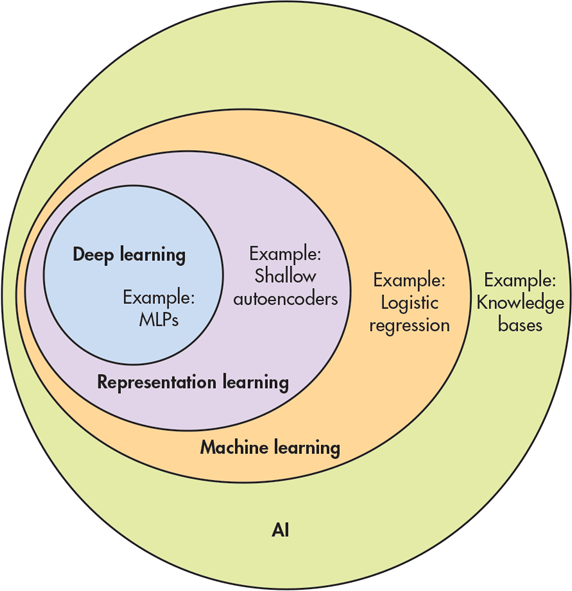
\includegraphics[width=0.276\textwidth]{figs/aiVennDiagram.png} \hspace{1cm}
    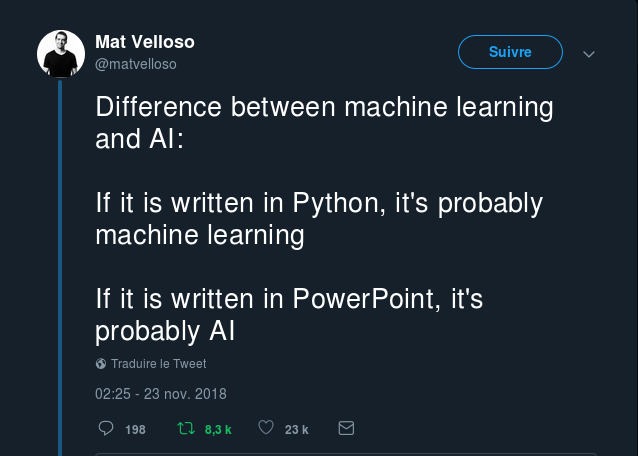
\includegraphics[width=0.4\textwidth]{figs/mlvsAI.png}
  \end{figure}
  \begin{itemize}
  \item \textcolor{agaetisOrange}{\textbf{AI}}: Domaine d'étude \boldmath $ \textcolor{agaetisOrange}{\Rightarrow}$ \unboldmath abus de langage (NN, RL)
  \item \textcolor{agaetisOrange}{\textbf{ML}}: Algorithmes/outils développés dans le cadre de la recherche sur l'IA
  \end{itemize}
\end{frame}

\begin{frame}{Machine Learning: Définitions}
    \begin{itemize}
  \item \textbf{\textcolor{agaetisOrange}{Arthur Samuel:}}
    \begin{itemize}
      \normalsize
    \item \textit{The field of study that gives computers the ability to learn without being explicitly programmed.}
    \end{itemize}
    \vspace{0.2cm}
  \item \textbf{\textcolor{agaetisOrange}{Tom Mitchell:}}
    \begin{itemize}
      \normalsize
    \item \textit{A computer program is said to learn from experience E with respect to some class of tasks T and performance measure P, if its performance at tasks in T, as measured by P, improves with experience E.}
    \end{itemize}
    \vspace{0.5cm}
  \item \textbf{\textcolor{agaetisOrange}{L'idée: }} Une machine apprend \textit{seule} à réaliser une tache complexe à l'aide de processus itératifs simple.
  \end{itemize}
\end{frame}

\begin{frame}{ML: Les principaux types d'apprentissage}
  \begin{minipage}{.1\textwidth}
  \end{minipage}
  \hfill
  \begin{minipage}{.75\textwidth}
    \begin{beamerboxesrounded}[scheme=suppervise,lower=box,width=0.8\textwidth]{\textcolor{black}{Supervisé}}
      \begin{itemize}
        \scriptsize
      \item Utilise des données \textit{labélisées}
      \item La machine apprend par l'exemple
      \item \textit{Prédis} le résultat pour de nouveaux événements
      \item Problèmes de prédictions et de classification
      \item Regression linéaire et logistique
      \item Réseaux de Neurones
      \item Arbres de décisions
      \end{itemize}
    \end{beamerboxesrounded}
  \end{minipage}
  \hfill
  \begin{minipage}{.1\textwidth}
  \end{minipage}

  \vfill
  
  \begin{minipage}{.48\textwidth}
    \begin{beamerboxesrounded}[scheme=suppervise,lower=box,width=0.95\textwidth]{\textcolor{black}{Non-supervisé}}
      \begin{itemize}
        \scriptsize
      \item Données non \textit{labélisées}
      \item La machine apprend par elle même à identifier une structure
      \item Évaluation des performances compliqué.
      \item Problèmes de classification, réduction de dimensions
      \item K-means
      \item Analyse en Composante Principale
      \end{itemize}
    \end{beamerboxesrounded}
  \end{minipage}
  \hfill
  \begin{minipage}{.48\textwidth}
    \begin{beamerboxesrounded}[scheme=suppervise,lower=box,width=0.95\textwidth]{\textcolor{black}{Par renforcement}}
      \begin{itemize}
        \scriptsize
        \vspace{0.7cm}
      \item Un agent A, effectue une action Ac, l'environnement E lui renvoie une récompense.
      \item Récompenses à court et long terme
      \item Utilisé par Deepmind (alphaGo)
        \vspace{0.7cm}
      \end{itemize}
    \end{beamerboxesrounded}
  \end{minipage}  
\end{frame}

\begin{frame}{À quelles problèmatiques répond le Machine Learning?}
  \begin{itemize}
  \item \textcolor{agaetisOrange}{\textbf{Prédictions}} Prédire une valeur continue à partir de caractéristique données
  \item \textcolor{agaetisOrange}{\textbf{Projections}} Prédictions spécifique de séries temporelles: $y = f(y(t-1), y(t-2), \dots)$
  \item \textcolor{agaetisOrange}{\textbf{Classifications}} Prédire la classe (discret) d'un objet en fonction de ses caractéristiques
  \item \textcolor{agaetisOrange}{\textbf{Segmentations}} Regrouper des objets par similarité dans l'espace des variables utilisé
  \item \textcolor{agaetisOrange}{\textbf{Compréhensions}} Comprendre l'importance de variables d'intérêt dans un contexte donné
  \end{itemize}
\end{frame}


\begin{frame}{La regression linéaire}
  \begin{itemize}
    
  \item Déterminer une relation \textit{linéaire} entre \textit{input(s)} (features) et \textit{output}:
    \begin{center}
      \normalsize
      \boldmath $\Rightarrow$ \unboldmath \textbf{\textcolor{agaetisOrange}{Apprentissage Supervisé}}
    \end{center}
  \item Prédiction d'une valeur \textbf{continue} (e.g. non discrète, non catégorielle)
  \item Applications:
    \begin{itemize}
      \normalsize
    \item Recherche de corrélations
    \item En science, modélisation de phénomènes (physiques, biologiques, ...) après mesures
    \item Dans le domaine médical: les études épidémiologique
    \item Dans la finance/économie: prédictions des tendances, \textit{Capital Asset Pricing Model}
    \item $\dots$
    \end{itemize}
  \end{itemize}
  \begin{center}
    \textbf{Sujet Data Science} \boldmath $\Rightarrow$ \unboldmath \textbf{Premier algorithme à tester!}
  \end{center}
\end{frame}

\begin{frame}{Un exemple: le prix d'une carte graphique}
  \begin{itemize}
  \item La propriété principale d'une carte Graphique: valeur de \textbf{GPU}
    \vspace{0.2cm}
  \item Jeu de données: $\{GPU;prix\}$:
  \end{itemize}

  \begin{figure}
    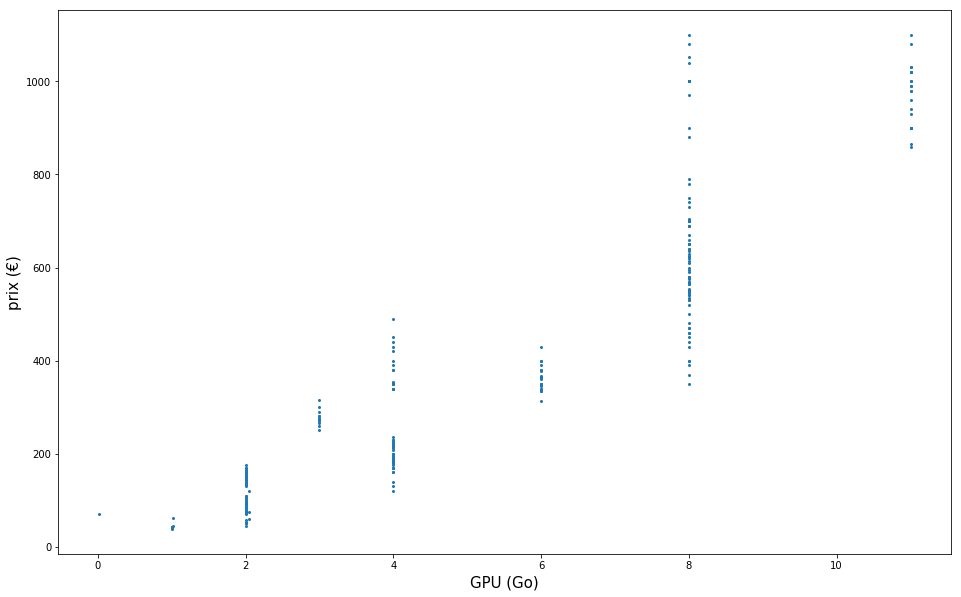
\includegraphics[width=0.5\textwidth]{figs/gpuPrices.png}    
  \end{figure}
\end{frame}

\begin{frame}{On peut maintenant faire une prédiction}
  \begin{itemize}
  \item Quel serait le prix de cartes avec 5, 10 et 14 Go de GPU? 
  \end{itemize}
  \vspace{-0.2cm}
  \begin{figure}
    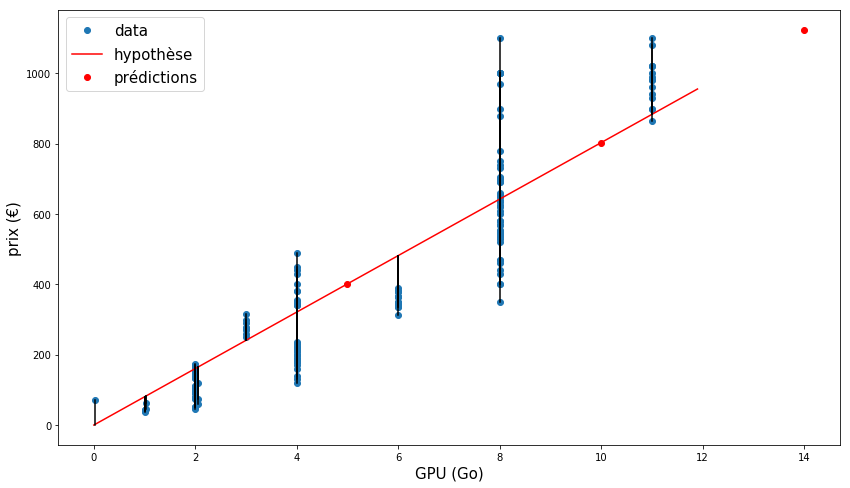
\includegraphics[width=0.6\textwidth]{figs/pred.png}
  \end{figure}
  \vspace{-0.5cm}
  \begin{itemize}
  \item On pourra les vendre autour de 400, 800 et 1100 euros!
  \end{itemize} 
\end{frame}

\begin{frame}{La regression linéaire multivariables}
  \begin{itemize}
    \item Le principe est le même, mais avec plusieurs variables $x_{i}$ (donc plusieurs paramètres $\theta_{i}$):
  \end{itemize}
    \begin{equation*}
      \hat{y} = \theta_{1}x_{1} + \dots + \theta_{n}x_{n} = \displaystyle\sum_{i=1}^{n} \theta_{i} x_{i}
    \end{equation*}
  \begin{figure}
    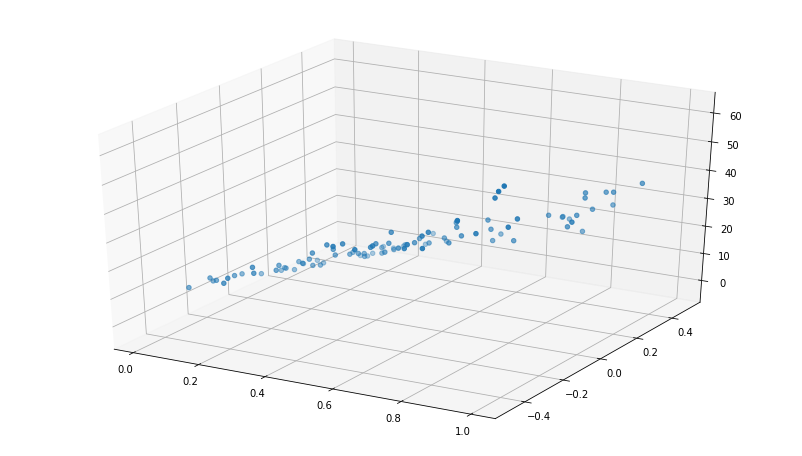
\includegraphics[width=0.45\textwidth]{figs/multiVarData.png}
    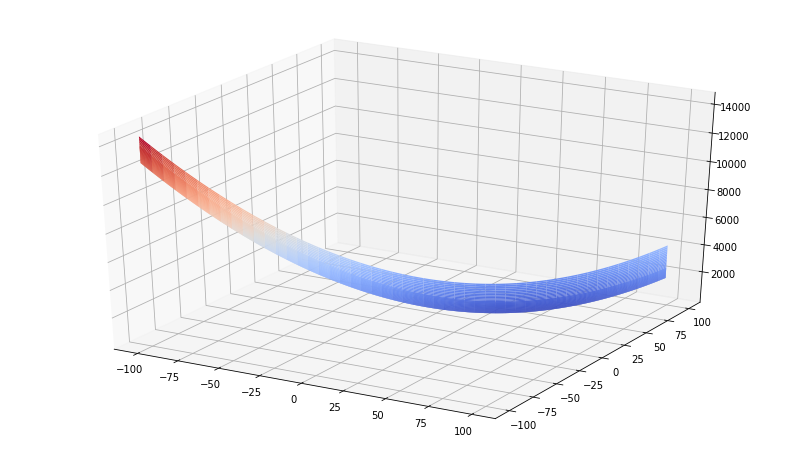
\includegraphics[width=0.45\textwidth]{figs/multiVarCostFct.png}\\
  \end{figure}
\end{frame}

\begin{frame}{Affinons notre modèle de carte graphiques}
  \begin{itemize}
  \item Plus de features: chipset, fréquence, consommation, ...
  \item Il va falloir explorer et nettoyer les données:
    \begin{itemize}
      \normalsize
    \item Gestion des données manquantes / abbérantes
    \item \textit{Features engineering}
    \item Normaliser le dataset (pour accélérer la descente de gradient)
    \end{itemize}
  \end{itemize}
\end{frame}

\begin{frame}{Régression linéaire multivariables: Résultats}
  \begin{itemize}
  \item Modèle simple: $err ~ \approx ~ 100$ (biais)
  \item Modèle multivariable: $err ~ \approx ~ 40 ~/~ 50$ (variance)
  \end{itemize}
  \begin{figure}
    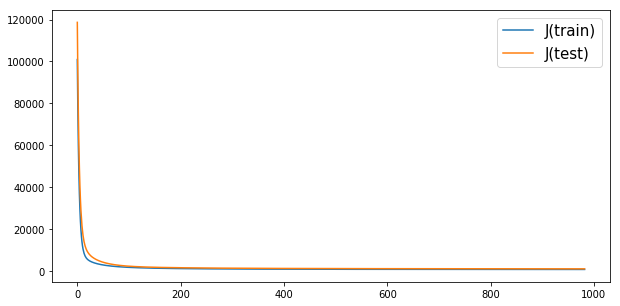
\includegraphics[width=0.45\textwidth]{figs/multiVarDesc.png}\\
  \end{figure}
\end{frame}
  
\begin{frame}{Pour conclure sur la régression linéaire}
  \begin{itemize}
  \item \textbf{Regression Linéaire:} $\hat{y}$ est une valeur \textit{continue}
    \begin{itemize}
    \item Valeur discrète: \textbf{Regression Logistique} (\textit{classification})
    \end{itemize}
    \vspace{0.2cm}
  \item Le résultat $\hat{y}$ dépend \textbf{linéairement} des variables $x_{i}$ si:
    \begin{equation*}
      \hat{y} = \theta_{1}x_{1} + \dots + \theta_{n}x_{n} = \displaystyle\sum_{i=1}^{n} \theta_{i} x_{i}
    \end{equation*}
  \item \textbf{Apprentissage supervisé}: $y$ est connu pour chaque $x_{1}$ dans le jeu de données d'entrainement
  \item Facile à implémenter (encore plus avec Scikit-learn ...), rapide: bon point de départ sur un sujet
  \end{itemize}
\end{frame}

\begin{frame}
  \begin{figure}
    
\includegraphics[width=0.5\textwidth]{figs/AGAETIS_GREY}
  \end{figure}
  \begin{center}
    \Large
    \textcolor{agaetisOrange}{Merci !}\\
    \large
    \textcolor{agaetisOrange}{Des questions?}\\
    \normalsize
    \vspace{0.5cm}
    Léo Beaucourt
  \end{center}
\end{frame}

\begin{frame}
  \textit{“There is a theory which states that if ever anyone discovers exactly what the Universe is for and why it is here, it will instantly disappear and be replaced by something even more bizarre and inexplicable.}\\
  \vspace{1cm}
  \textit{There is another theory which states that this has already happened.”}\\
  \vspace{1cm}
  \hfill Douglas Adams
\end{frame}

\end{document}
